\chapter{Ablauf der Fallstudie}\label{sec:fallstudie}

Da die Testautomatisierung bei einem verteilten, adaptiven System sehr aufwändig werden kann, soll nun ein modellbasierter Ansatz genutzt werden. Als reales System wurde Apache\texttrademark Hadoop\textregistered\footnote{\url{https://hadoop.apache.org/}} ausgewählt, welches mit einer adaptiven Komponente erweitert wurde. Von Hadoop sollen nun einige relevante Komponenten als Modell nachgebildet werden und anschließend mit einem realen Hadoop-Cluster verbunden werden. Dadurch soll der Ansatz des modellbasierten Testen auf ein reales System übertragen werden.
%Bei der Umsetzung spielen einige Hauptprobleme wie \zB die Einbindung des realen Systems in das Modell oder der Umgang mit asynchronen Prozessen bei verteilten Systemen ebenfalls eine Rolle.

\input{./fallstudie/ablauf}

\section{Apache Hadoop}\label{sec:hadoop}

\textbf{Apache Hadoop} ist ein Open-Source-Software-Projekt, mit dessen Hilfe ermöglicht wird, Programme zur Datenverarbeitung mit großen Ressourcenbedarf auf verteilten System auszuführen. Hadoop wird von der \emph{Apache Foundation} entwickelt und bietet verschiedene Komponenten an, welche vollständig skalierbar sind, von einer einfachen Installation auf einem PC bis hin zu einer Installation über mehrere Server in einem Serverzentrum. Hadoop besteht hauptsächlich aus folgenden Kernmodulen \cite{HadoopHomePage}:

\begin{description}
	\item[Hadoop Common] Gemeinsam genutzte Kernkomponenten
	\item[Hadoop YARN] Framework zur Verteilung und Ausführung von Anwendungen und das dazugehörige Ressourcen-Management
	\item[Hadoop Distributed File System] Kurz HDFS, Verteiltes Dateisystem
	\item[Hadoop MapReduce] YARN-Basiertes System zum Verarbeiten von großen Datenmengen
\end{description}

Hadoop ermöglicht es dadurch, sehr einfach mit Anwendungen umzugehen, welche große Datenmengen verarbeiten. Da es für Hadoop nicht relevant ist, auf wie vielen Servern es läuft, kann es beliebig skaliert werden, wodurch entsprechend viele Ressourcen zur Bearbeitung und Speicherung von großen Datenmengen zur Verfügung stehen können.

\begin{figure}
	\centering
	\includegraphics[width=\columnwidth]{./images/yarn_architecture.png}
	\caption[Architektur von YARN]{Architektur von YARN (entnommen aus \cite{HadoopYarnArch271})}
	\label{fig:yarnarch}
\end{figure}

Die Kernidee der Architektur von \textbf{YARN} ist die Trennung vom Ressourcenmanagement und Scheduling. Dazu besitzt der Master bzw. \emph{Controller} den \ac{RM}, welcher für das gesamte System zuständig ist und die Anwendungen im System verteilt und überwacht und somit auch als \emph{Load-Balancer} agiert. Er besteht aus zwei Kernkomponenten, dem \ac{AM} und dem \emph{Scheduler}. Der \ac{AM} ist für die Annahme und Ausführung von einzelnen Anwendungen zuständig, denen der Scheduler die dafür notwendigen Ressourcen im Cluster zuteilt.

Jeder Slave-\emph{Node} im Hadoop-Cluster besitzt einen \ac{NM}, welcher für die Überwachung der Ressourcen des Nodes und der darauf ausgeführten Anwendungs-Container zuständig ist und diese dem \ac{RM} mitteilt.

Jede YARN-Anwendung bzw. Job besteht aus einem oder mehreren Ausführungsversuchen, genannt \emph{Attempts}, denen wiederum mehrere \emph{Container} zugeordnet sind. Container können auf einem beliebigen Node ausgeführt werden und repräsentieren die Ausführung eines Tasks der Anwendung. Ein besonderer Container bildet dabei der \ac{AppMstr}, welcher innerhalb seines Attempts für das anwendungsbezogene Monitoring und die Kommunikation mit dem \ac{RM} und \ac{NM} zuständig ist und die dazu notwendigen Informationen bereit stellt \cite{HadoopYarnArch271}.

Hadoop enthält zudem einen sog. \ac{TLS}. Er ist speziell dafür entwickelt, die Metadaten und Logs der YARN-Anwendungen zu speichern und jederzeit, also auch als Anwendungshistorie, auszugeben \cite{HadoopYarnTlServer271}.

\begin{figure}
    \centering
    \includegraphics[width=.8\columnwidth]{./images/hdfsarchitecture.png}
    \caption[Architektur des HDFS]{Architektur des HDFS (entnommen aus \cite{HadoopHdfsDesc271})}
    \label{fig:hdfsarch}
\end{figure}

Das \textbf{HDFS} basiert auf der gleichen Architektur wie YARN und besitzt ebenfalls einen Master und mehrere Slaves, welches in der Regel die gleichen Nodes sind wie bei YARN sind. Der \emph{NameNode} ist als Master für die Verwaltung des Dateisystems zuständig und reguliert den Zugriff auf die darauf gespeicherten Daten. Die Daten selbst werden in mehrere Blöcke aufgeteilt auf den \emph{DataNodes} gespeichert. Um den Zugriff auf die Daten im Falle eines Node-Ausfalls zu gewährleisten, wird jeder Block auf anderen Nodes repliziert. Dateioperationen (wie Öffnen oder Schließen) werden direkt auf den DataNodes ausgeführt, sie sind darüber hinaus auch dafür verantwortlich, dass Clients die Daten lesen oder beschreiben können \cite{HadoopHdfsDesc271}.

\textbf{MapReduce} bietet analog zu YARN die Möglichkeit, Anwendungen mit einem großen Ressourcenbedarf, welche große Datenmengen verarbeiten, auf einem gesamten Cluster auszuführen. Dazu werden bei einem MapReduce-Job die Eingabedaten aufgeteilt, anschließend von den sog. \emph{Map Tasks} verarbeitet und deren Ausgaben von den sog. \emph{Reduce Tasks} geordnet. Für die Ein- und Ausgabe der Daten wird in der Regel das HDFS, für die Ausführung der einzelnen Tasks YARN genutzt \cite{HadoopMapRedTutorial271}. MapReduce kann auch als Vorgänger von YARN angesehen werden, da YARN auch als \emph{MapReduce Next Gen} bzw. \emph{MRv2} bezeichnet wird und aufgrund der API-Kompatibilität von YARN jede MapReduce-Anwendung in der Regel auch auf YARN ausgeführt werden kann \cite{HadoopYarnArch271,HadoopYarnOverview271}.


\section{Adaptive Komponente in Hadoop}\label{sec:inriaSetting}

Ein normales Hadoop besitzt von Haus aus keine adaptive Komponente, sondern rein statische Einstellungen. Um damit Hadoop zu optimieren, müssen die Einstellungen immer manuell auf den jeweils benötigten Anwendungstyp angepasst werden. Dazu gibt es auch bereits verschiedene Scheduler, den \emph{Fair Scheduler}, welcher alle Anwendungen ausführt und ihnen gleich viele Ressourcen zuteilt, und den \emph{Capacity Scheduler}. Letzterer sorgt dafür, dass nur eine bestimmte Anzahl an Anwendungen pro Benutzter gleichzeitig ausgeführt wird und teilt ihnen so viele Ressourcen zu, wie benötigt werden bzw. der Benutzter nutzen darf. Entwickelt wurde der Capacity Scheduler vor allem für Cluster, die von mehreren Organisationen gemeinsam verwendet werden und sicherstellen soll, dass jede Organisation eine Mindestmenge an Ressourcen zur Verfügung hat \cite{HadoopCapScheduler271}.

Je nach Bedarf besitzt der Capacity Scheduler entsprechende Einstellungen, um \zB den verfügbaren Speicher pro Container festzulegen. Eine weitere Einstellung des Schedulers ist \texttt{maximum-am-resource-percent}, auch MARP genannt, der angibt, wie viele Prozent der gesamten Ressourcen durch \ac{AppMstr} genutzt werden dürfen \cite{HadoopCapScheduler271}. Damit bewirkt diese Einstellung indirekt auch die maximale Anzahl an Anwendungen, die gleichzeitig ausgeführt werden dürfen. Da der MARP-Wert jedoch nicht während der Laufzeit dynamisch angepasst werden kann, haben \citeauthor{zhang2016} in \cite{zhang2016} einen Ansatz zur dynamischen Anpassung des MARP-Wertes zur Laufzeit von Hadoop vorgestellt. Dadurch wird der MARP-Wert abhängig von den ausgeführten Anwendungen adaptiv zur Laufzeit angepasst, sodass immer möglichst viele Anwendungen gleichzeitig ausgeführt werden können. Gemäß \citeauthor{zhang2016} werden dadurch Anwendungen im Schnitt um bis zu 40 \% schneller ausgeführt.

\begin{figure}
    \centering
    \includegraphics[width=.8\columnwidth]{./images/marpValue.pdf}
    \caption[LoJP und LoJT in Hadoop]{LoJP und LoJT in Hadoop \cite{zhang2016}}
    \label{fig:marpValue}
\end{figure}

Der Hintergrund dieser \emph{Selfbalancing-Komponente} ist der, dass durch den MARP-Wert der für die Anwendungen verfügbare Speicher in zwei Teile aufgeteilt wird. Im einen Teil befinden sich alle derzeit ausgeführten \ac{AppMstr}, im anderen Teil die von den Anwendungen benötigten weiteren Container. Wie groß der Teil für die \ac{AppMstr} ist, wird nun durch den MARP-Wert bestimmt. Ist der MARP-Wert zu klein, können nur wenige \ac{AppMstr} (und damit Anwendungen) gleichzeitig ausgeführt werden (\emph{Loss of Jobs Parallelism}, LoJP). Ist der MARP-Wert jedoch zu groß, können für die ausgeführten Anwendungen nur wenige Container bereitgestellt werden, wodurch sich die Ausführung für eine Anwendung wesentlich verlangsamt (\emph{Loss of Job Throughput}, LoJT)\cite{zhang2016}.

Die Selfbalancing-Komponente passt daher den MARP-Wert abhängig von der Speicherauslastung dynamisch zur Laufzeit an. So wird der MARP-Wert verringert, wenn die Speicherauslastung sehr hoch ist, und erhöht, wenn die Speicherauslastung sehr niedrig ist \cite{zhang2016}. Dadurch wird es ermöglicht, dass die maximal mögliche Anzahl an Anwendungen ausgeführt werden kann. Die Evaluation von \citeauthor{zhang2016} ergab zudem, dass die dynamische Anpassung des MARP-Wertes zudem auch effizienter ist als eine manuelle, statische Optimierung.


\section{Umsetzung des realen Clusters}\label{sec:aufbauCluster}

\citeauthor{zhang2016} haben im Rahmen ihrer gesamten Forschungsarbeit die Open"=Source"=Plattform Hadoop"=Benchmark entwickelt und auf Github zur Verfügung gestellt.\footnote{\url{https://github.com/Spirals-Team/hadoop-benchmark}}
Sie wurde speziell zum Einsatz in der Forschung erstellt und kann jederzeit an die eigenen Bedürfnisse angepasst werden.
Auf Basis dieser Plattform und der enthaltenen Benchmarks wurde das reale Cluster für diese Masterarbeit aufgebaut.

\subsection{Plattform Hadoop"=Benchmark}\label{sec:hadoopBenchmark}

Die Plattform ist in mehrere Szenarien unterteilt, darunter ein Hadoop in der Version 2.7.1 ohne Änderungen und ein darauf basierendes Szenario mit der Selfbalancing"=Komponente.
Hadoop"=Benchmark basiert auf der Software \emph{Docker}\footnote{\url{https://www.docker.com/}} und dem dazugehörigen Tool \emph{Docker Machine}, um damit mit wenigen Befehlen ein Hadoop"=Cluster aufbauen zu können.
Mit \emph{Graphite}\footnote{\url{https://graphiteapp.org/}} ist zudem ein Monitoring"=Tool enthalten, mit dem die Systemwerte wie CPU- oder Speicher"=Auslastung des Clusters überwacht und analysiert werden kann.

\begin{figure}
    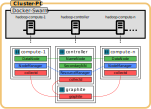
\includegraphics{./images/hadoopBenchmarkArch.png}
    \caption[High"=Level"=Architektur von Hadoop"=Benchmark]
    {High"=Level"=Architektur von Hadoop"=Benchmark.
        Entnommen aus \cite{abb:hadoopBenchmarkArch}.}
    \label{fig:hadoopBenchmarkArchitecture}
\end{figure}

\autoref{fig:hadoopBenchmarkArchitecture} zeigt die grundlegende Architektur der Plattform, die mithilfe eines Docker"=Swarms auf mehreren \emph{Docker Machines} ein Cluster erstellt, auf denen dann in den Docker"=Containern das eigentliche Hadoop"=Cluster ausgeführt wird.
In Hadoop"=Benchmark werden mithilfe von Docker"=Machine und VirtualBox\footnote{\url{https://www.virtualbox.org/}} virtuelle Maschinen erstellt, die mit dem  Betriebssystem \emph{Boot2Docker} ausgestattet sind.
Boot2Docker ist eine leichtgewichtige Linux"=Distribution, auf der Docker bereits vorinstalliert ist \cite{DockerMachineGettingStartedVm}.
Jeder Hadoop"=Container enthält zudem das Tool \emph{collectd}\footnote{\url{https://collectd.org/}}, was das Monitoring des Containers auf Systemebene übernimmt und die Daten an den Graphite"=Container übermittelt.
Dadurch wird es möglich, eine beliebige Anzahl an voneinander unabhängigen Nodes auf einem physischen Computer ausführen zu können.
Auch ist es möglich, den Docker"=Machines einen beliebig großen Arbeitsspeicher zur Verfügung zu stellen.

Die Plattform Hadoop"=Benchmark enthält zudem einige Benchmark"=Anwendungen:

\begin{itemize}
    \item Hadoop Mapreduce Examples
    \item Intel HiBench\footnote{\url{https://github.com/intel-hadoop/HiBench}}
    \item \ac{SWIM} \footnote{\url{https://github.com/SWIMProjectUCB/SWIM}}
\end{itemize}

Eine Besonderheit bildet der SWIM"=Benchmark, welcher sehr Ressourcenintensiv ist und daher auf einem \emph{Single Node Cluster}, also einem kompletten Hadoop"=Cluster auf nur einem Computer, sehr zeitintensiv sein kann.
Der Intel HiBench"=Benchmark besteht aus Kategorien wie \emph{Machine Learning} oder Graphen, welche wiederum aus einen oder mehreren \emph{Workloads} bestehen, welche entsprechende Anwendungen bzw. Algorithmen auf dem Hadoop"=Cluster ausführen.
Einige der Hibench"=Workloads basieren auf den Mapreduce Examples, welche wiederum voneinander unabhängige Beispielanwendungen für Hadoop darstellen.

\subsection{In dieser Fallstudie verwendetes Setup}\label{sec:clusterFallstudie}

Da die Plattform Hadoop"=Benchmark mithilfe von Docker auf einem physischen PC sehr einfach ein komplettes Hadoop"=Cluster ausführen kann, wurde die Plattform für diese Fallstudie als Basis genutzt.
Da Docker und Hadoop vor allem für den Einsatz in einer Linux"=Umgebung entwickelt wurden, werden für die Fallstudie zwei Computer genutzt, auf denen das Cluster wahlweise auf einem oder auf beiden Hosts ausgeführt werden kann.
Zudem wird auf einem Host eine VM mit Windows 10 ausgeführt, das zum Ausführen des .NET"=Frameworks bzw. \sS benötigt wird.
Beide zum Einsatz kommenden Hosts sind jeweils mit einem Intel Core i5"=4570 @ 3,2 GHz x 4, 16 GB Arbeitsspeicher sowie einer SSD ausgestattet, auf der Ubuntu 16.04 LTS installiert ist.
Die Verbindung von Windows zu Linux auf beiden Hosts wird mithilfe von SSH"=Verbindungen umgesetzt.

\begin{figure}
    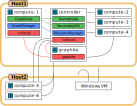
\includegraphics{./images/caseStudyHadoopSetup.pdf}
    \caption[In der Fallstudie verwendetes Cluster"=Setup]
    {In der Fallstudie verwendetes Cluster"=Setup.
        Grün: \ac{HDFS}, Blau: YARN, Rot: Graphite.}
    \label{fig:caseStudyHadoopSetup}
\end{figure}

\todo{Irgendwo erwähnen, wie Docker-Container aufeinander aufbauen}
Die beiden Abbildungen \autoref{fig:hadoopBenchmarkArchitecture} und \autoref{fig:caseStudyHadoopSetup} zeigen bereits den großen Hauptunterschied zwischen der Plattform und dem hier verwendeten Cluster"=Setup.
Da durch die Nutzung von virtuellen Maschinen ein zusätzlicher Ressourcenbedarf entsteht, wird im hier verwendeten Setup darauf verzichtet.
Durch die Ausführung der Docker"=Container des Hadoop"=Clusters direkt auf dem Host stehen dem Cluster mehr Ressourcen zur Verfügung.
Zudem wird es mithilfe von von \emph{Docker Swarm} so ermöglicht, das Hadoop"=Cluster auf beiden Hosts auszuführen.
Im konkreten Setup werden dabei Graphite, der Hadoop"=Controller sowie vier Hadoop"=Nodes auf dem Host1, sowie zwei weitere, optionale Nodes auf Host2 ausgeführt.
Weitere Anpassungen des verwendeten Setups bestehen \uA darin, dass der \ac{TLS} von Hadoop ebenfalls gestartet wird.
Zudem wurden einige Einstellungen von Hadoop so angepasst, dass defekte Nodes schneller erkannt werden.

Zum Ausführen der Windows"=VM auf Host2 wird VirtualBox 5.2 verwendet.
Zum Abrufen von Daten mithilfe der REST"=API von Hadoop über die SSH"=Verbindungen wird \emph{curl}\footnote{\url{https://curl.haxx.se/}} genutzt.
Zum Ausführen des Hadoop"=Clusters wird Docker in der Version 18.03 CE genutzt.

Um die in dieser Fallstudie benötigten Befehle einfach ausführen zu können, wurden zwei eigene Scripte erstellt, welche zum Teil auf den bestehenden Scripten der Plattform aufbauen.
Das Setup"=Script dient für folgende Zwecke:

\begin{itemize}
    \item Starten und Beenden des Clusters
    \item Starten und Beenden einzelner Hadoop"=Nodes
    \item Hinzufügen und Entfernen der Netzwerkverbindung des Docker"=Containers eines Hadoop"=Nodes
    \item Ausführen von eigenen Befehlen auf dem Docker"=Container des Hadoop"=Controllers
    \item Erstellen des Hadoop"=Docker"=Images
\end{itemize}

Das zweite erstellte Script dient ausschließlich zum Starten der Benchmarks.
Dazu werden die in der Plattform bereits enthaltenen Start"=Scripte aufgerufen, die für das konkrete Setup angepasst wurden.
